\begin{figure}[htb]
    \centering
    \begin{subfigure}{.3\textwidth}
        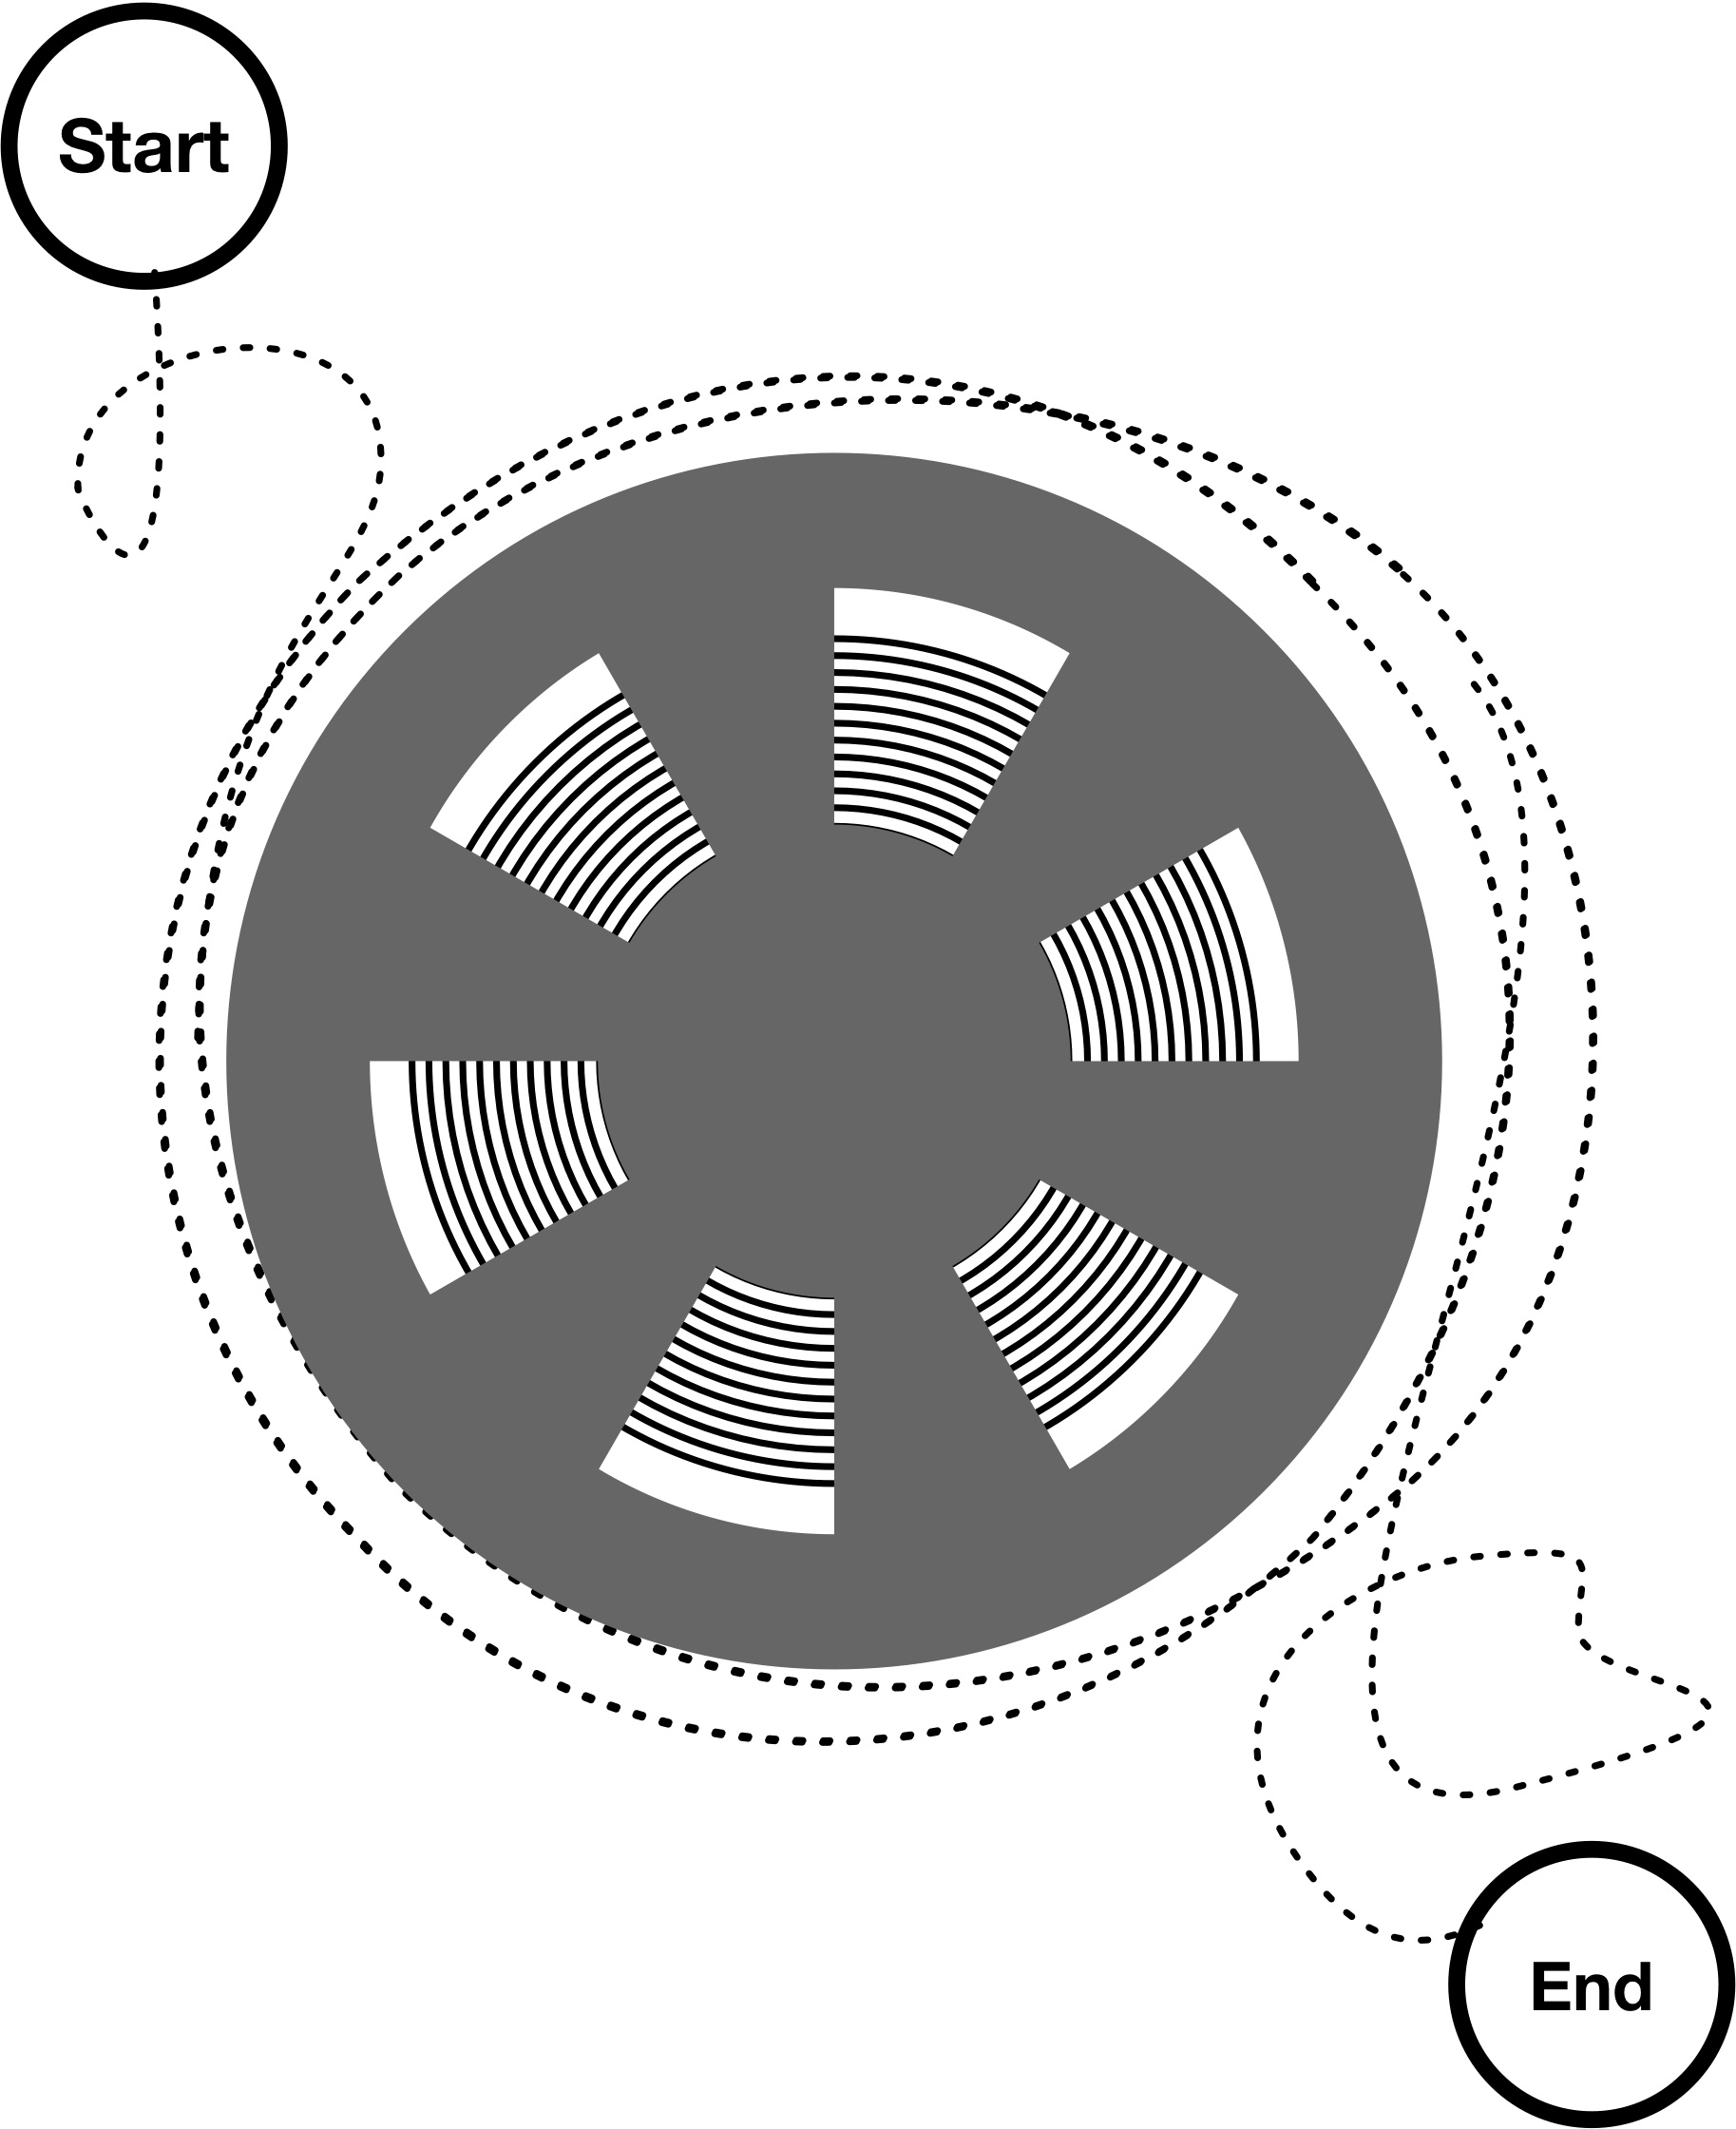
\includegraphics[width=\textwidth]{loose-spool.jpg}
        \caption{\label{fig:loose-spool}}
    \end{subfigure}
    \begin{subfigure}{.3\textwidth}
        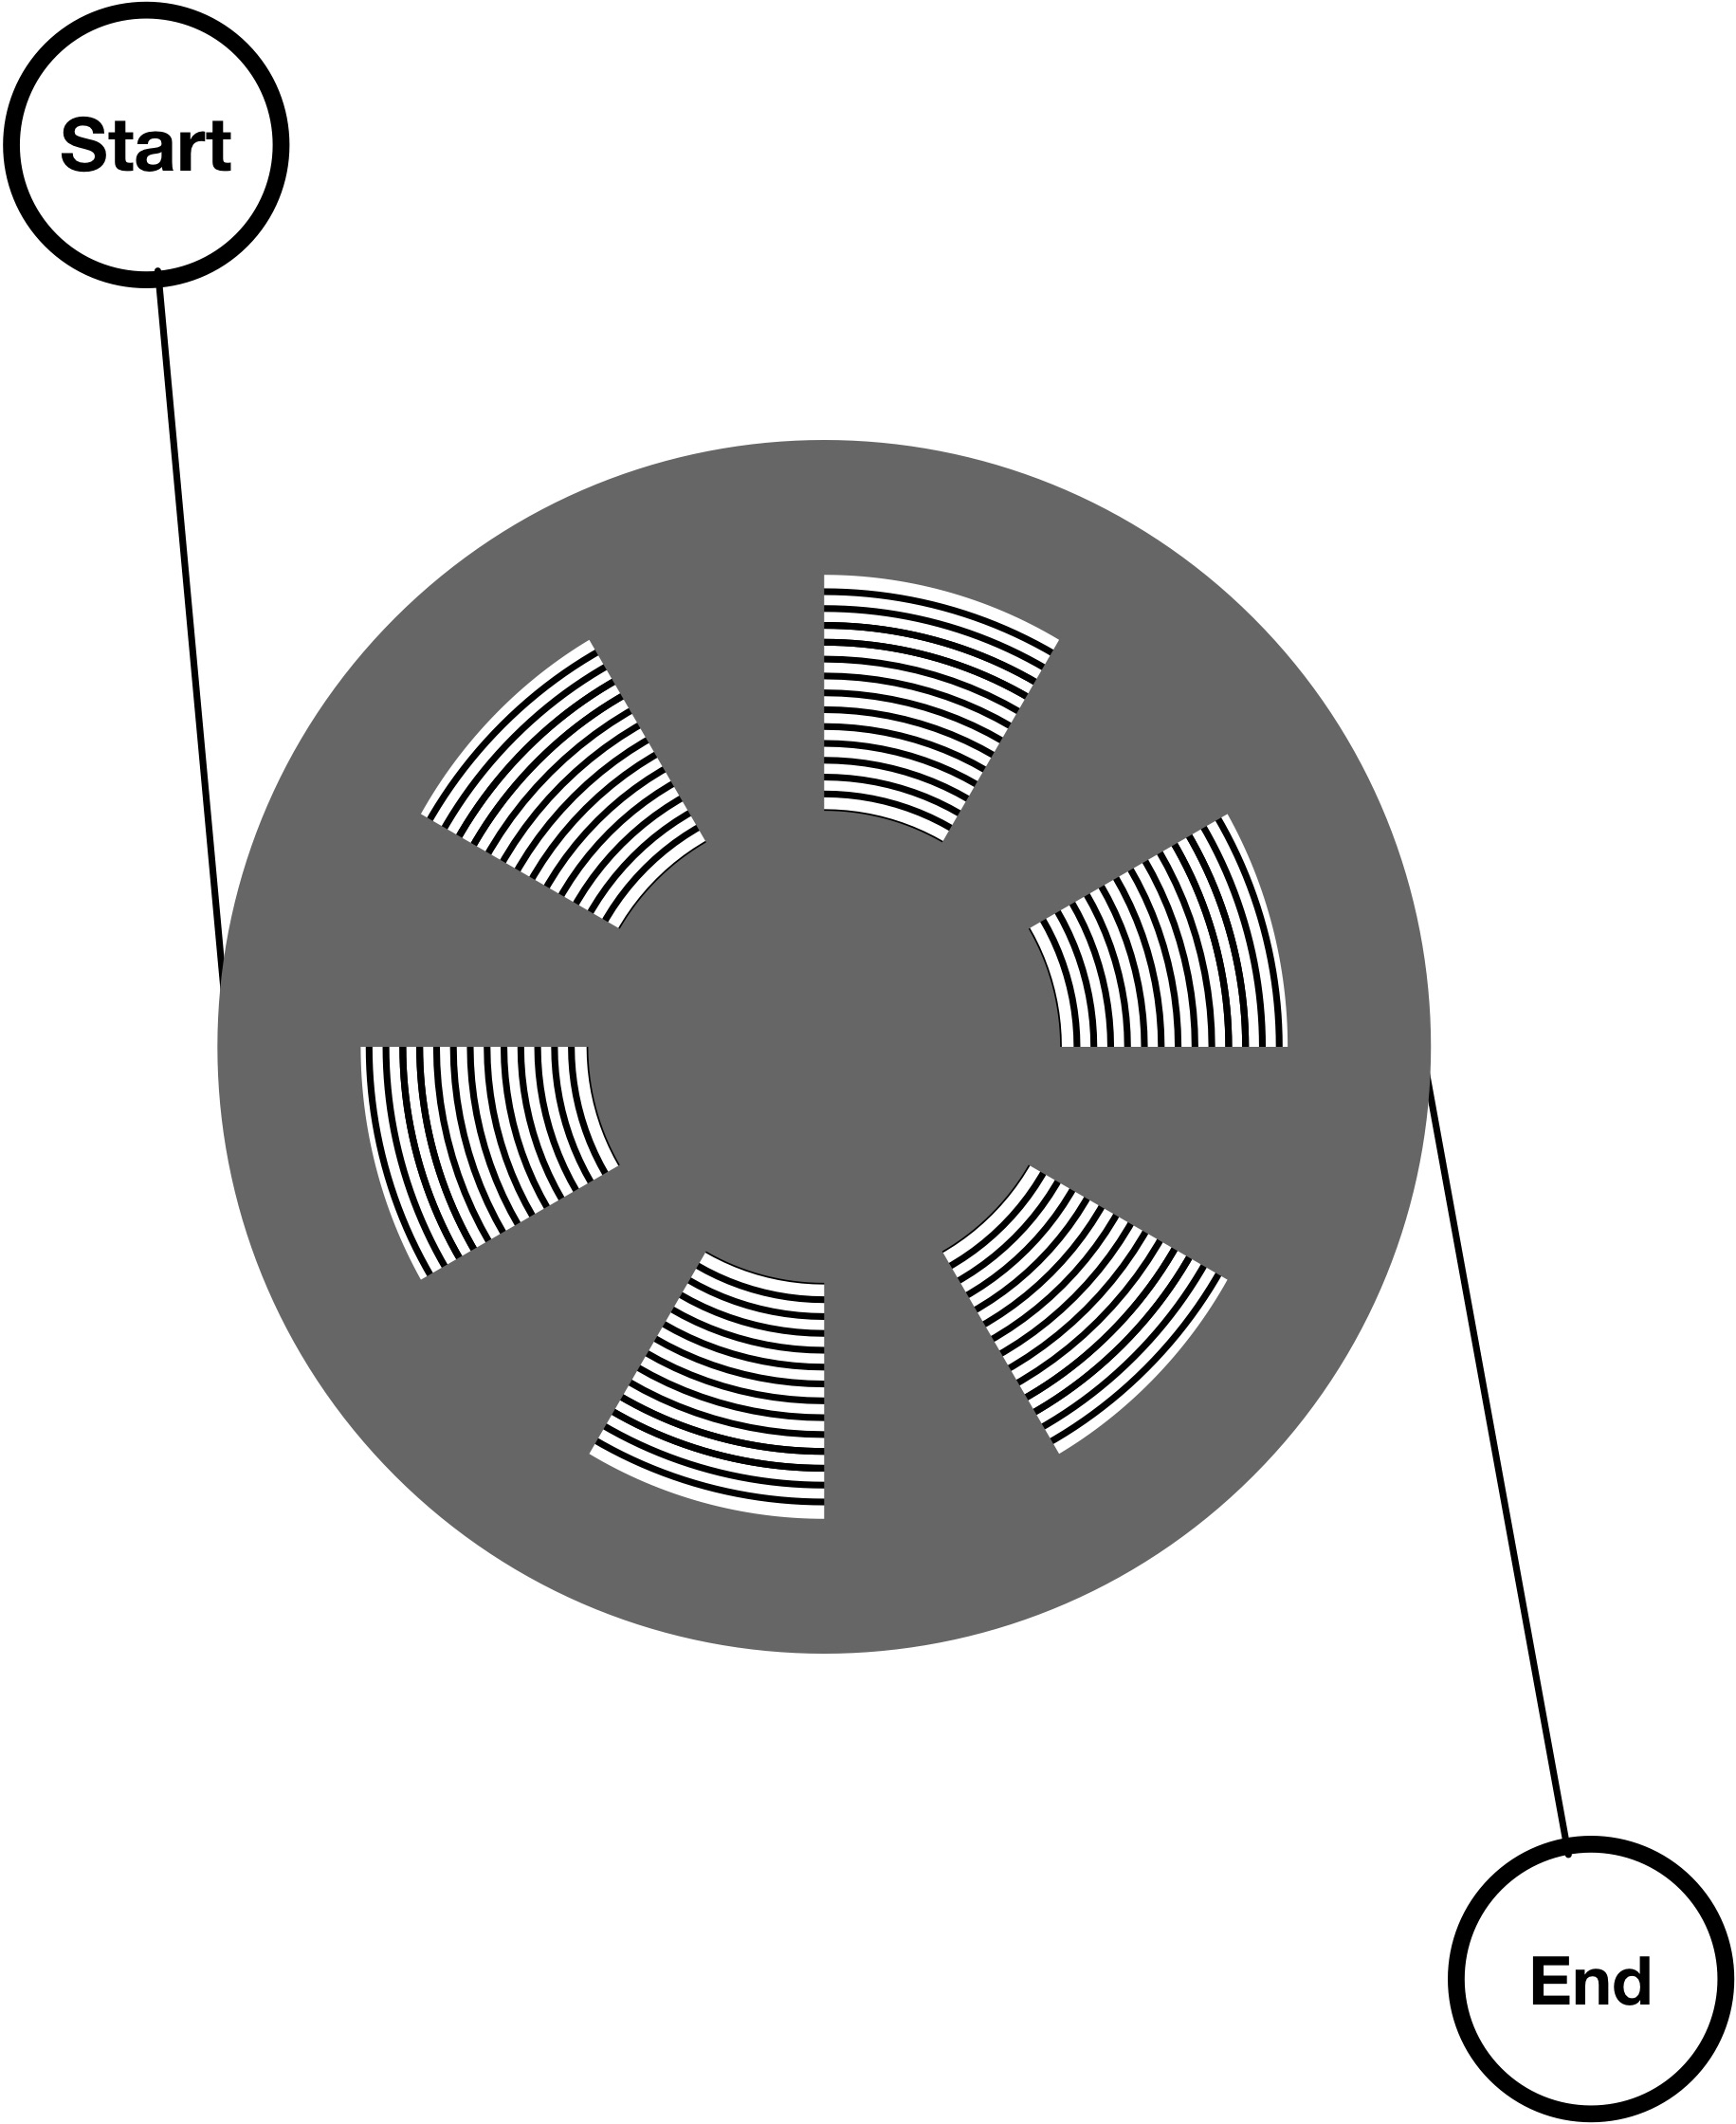
\includegraphics[width=\textwidth]{tight-spool.jpg}
        \caption{\label{fig:tight-spool}}
    \end{subfigure}
    \caption{\label{fig:spool-loop} Using spool as a metaphor for loop in program,
    duplicate code around a loop would be like tightening messy yarns into neat spool.
    `Loop rotation' can be pictorially depicted as winding up loose yarns onto a spool.
    \protect\subref{fig:loose-spool}: Duplicate, sloppy code is analogous to loose, unorganized
    yarn around a spool.
    \protect\subref{fig:tight-spool}: A neat loop is analogous to a tidy spool.}
\end{figure}


Coming with the productivity amplification power is the coding complexity of loops.
There are two key observations about loops.
First, a loop seldom lives in vacuum.
Loops are often used as an embedded subunits in a program just like an organelle in a living cell.
So it has to get along with its neighbors.
As a result, a large part of loop programming is to ``fit it in''.
Secondly, there are many moving parts in a loop construct and they are tightly coupled, changes in
one necessarily demand changes in others.
As we discussed in ~\autoref{sec:introduction}, the biggest problem with loop programming is
duplicate code in and around the loop.
The foremost goal in implementing loop is to reduce duplicate code.
`Loop rotation' is an important technique for that purpose.


As a helpful analogy, it is beneficial to visualize a loop construct as a spool.
Loops are to program as spools are to yarn---just as spools are used to organize yarn, loops are
invented to organize program.
From this perspective, the `loop rotation' process to coalesce duplicate code is analogous to
wind up loose and messy yarn into a tidy spool (~\autoref{fig:spool-loop}).


Additionally, a loop may be pictured as a Ferris wheel, a carousel and so on among which
the shared property is the symmetry with respect to circular shifts.
Aside from the point of entrance and one or more exits, a loop may be mathematically
represented by a circular sequence, that is, a sequence with rotational symmetry.
One can thus take this rotational degrees of freedom to one's advantage to decide where
to enter and where to exit the loop.


\begin{figure}[htb]
    \centering
    \begin{subfigure}{.3\textwidth}
        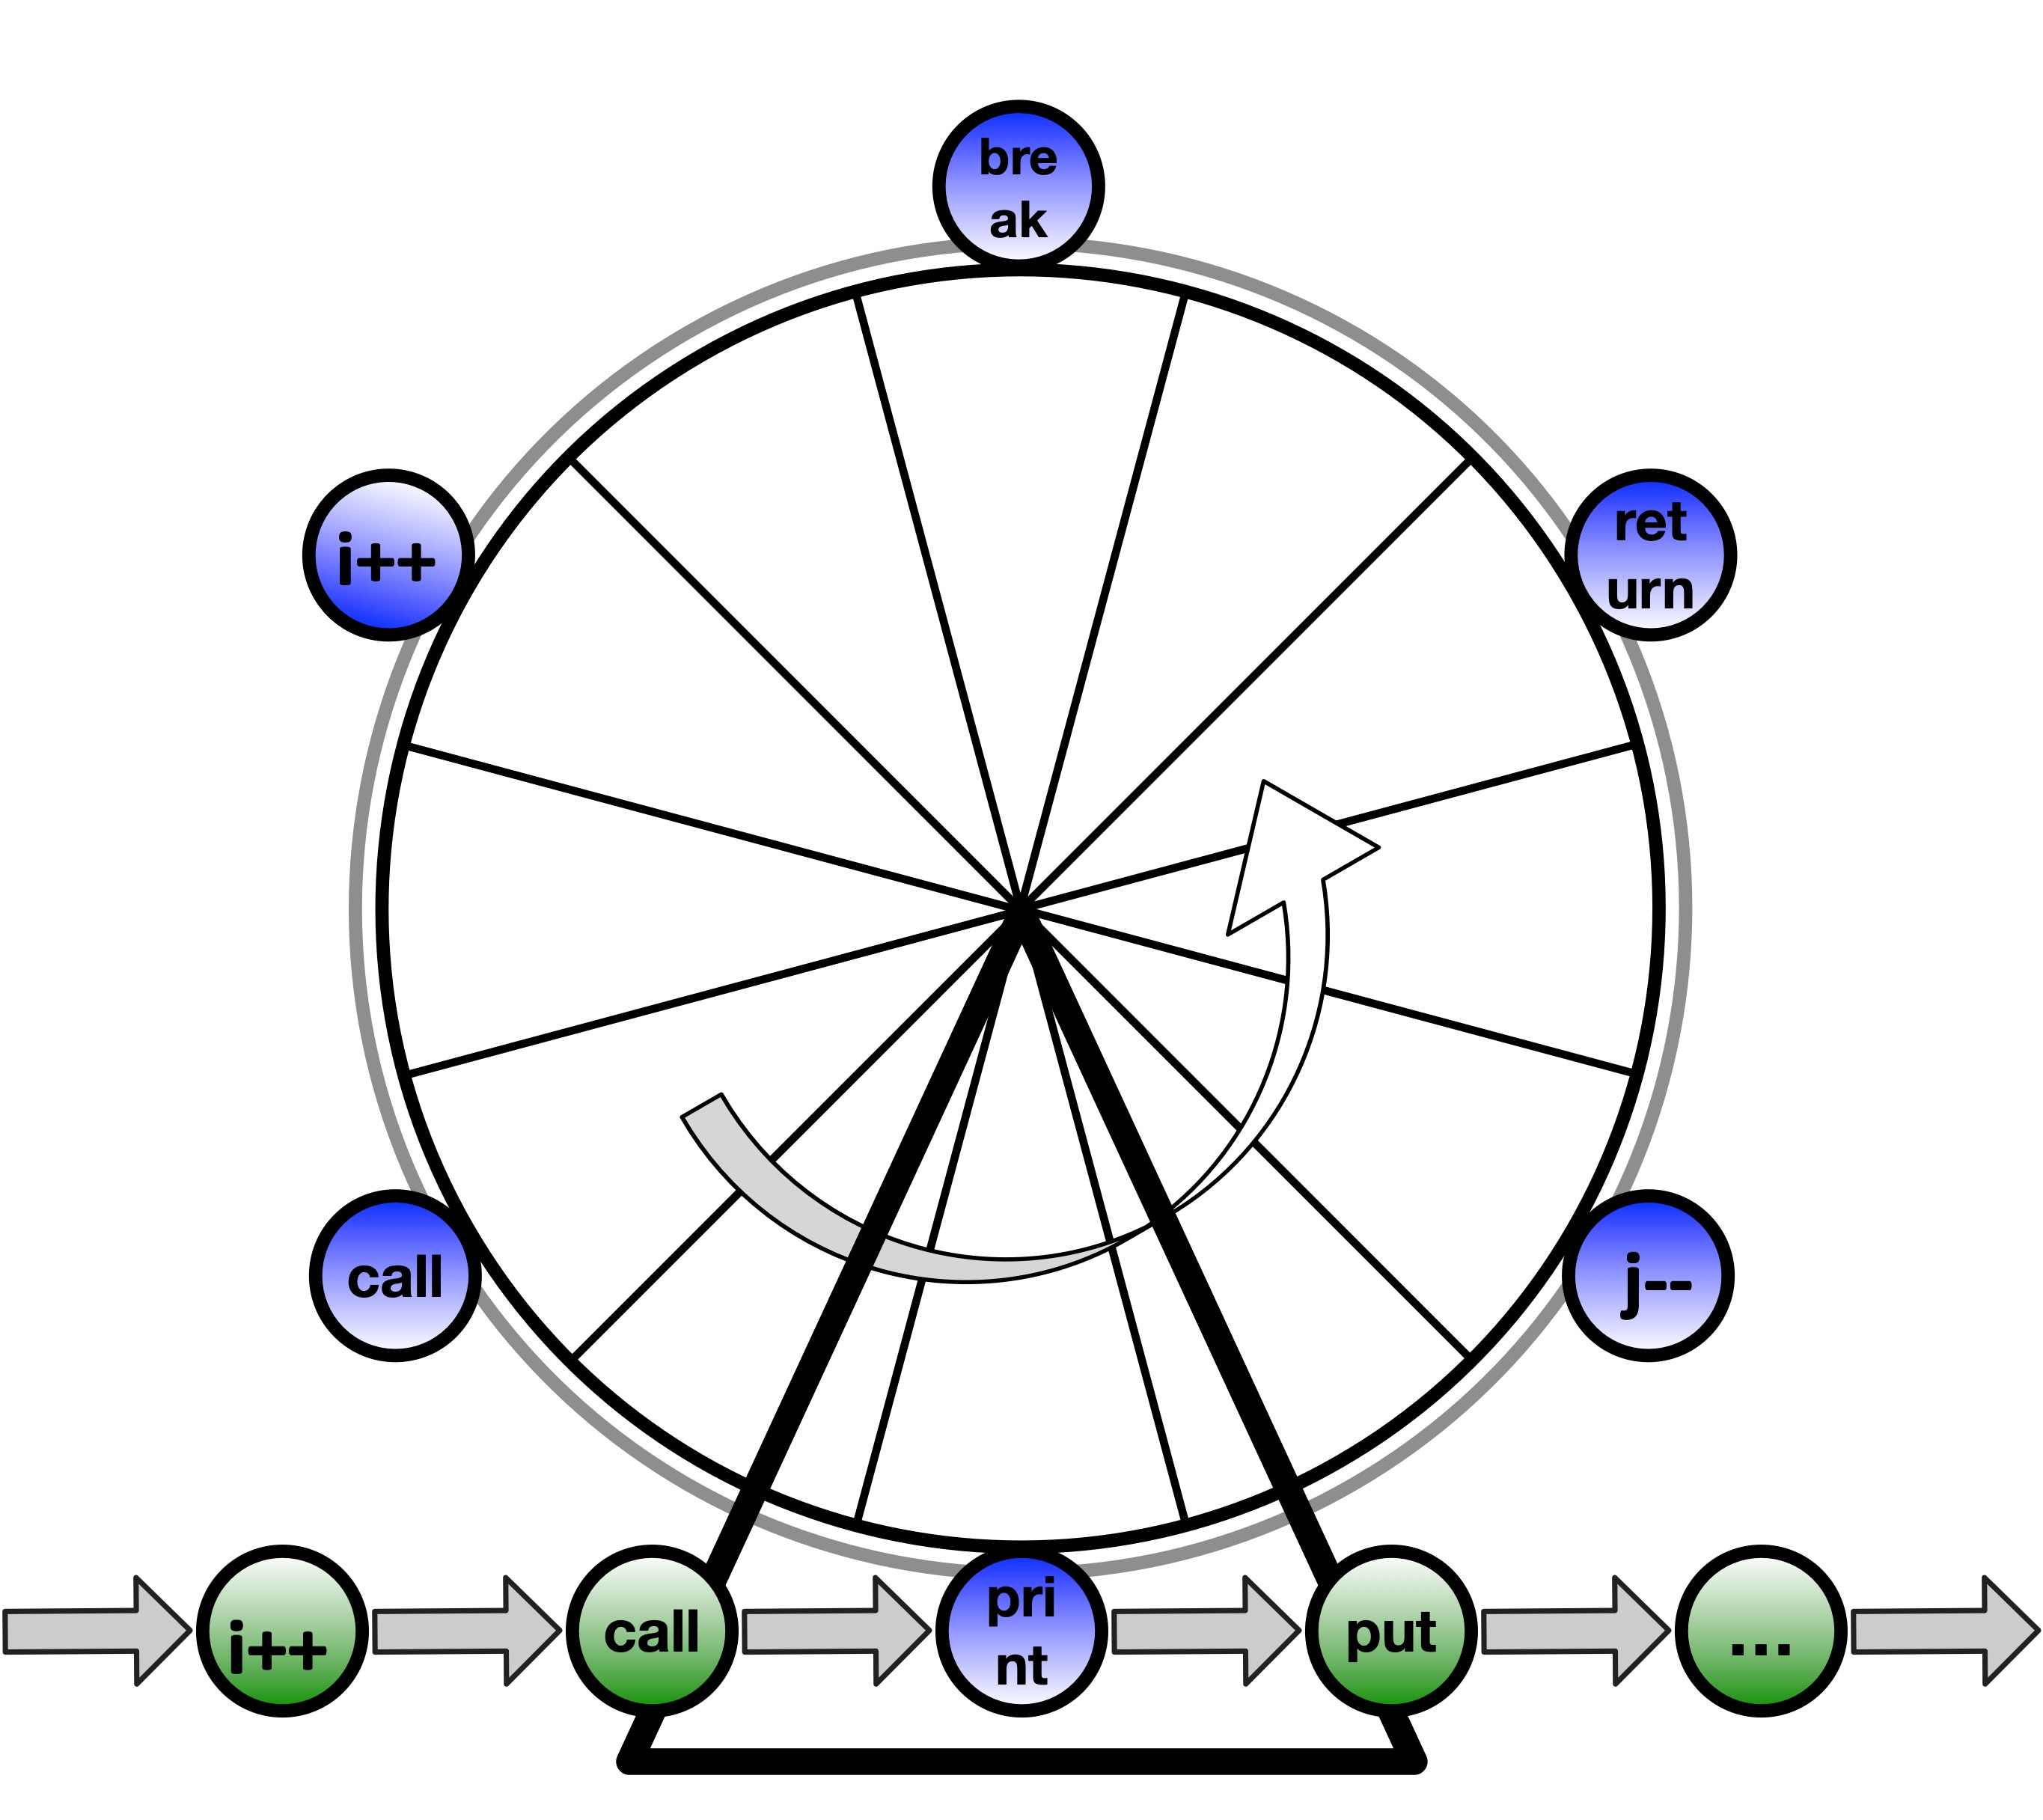
\includegraphics[width=\textwidth]{ferris-wheel.jpg}
        \caption{\label{fig:ferris-wheel-dup-node}}
    \end{subfigure}
    \begin{subfigure}{.3\textwidth}
        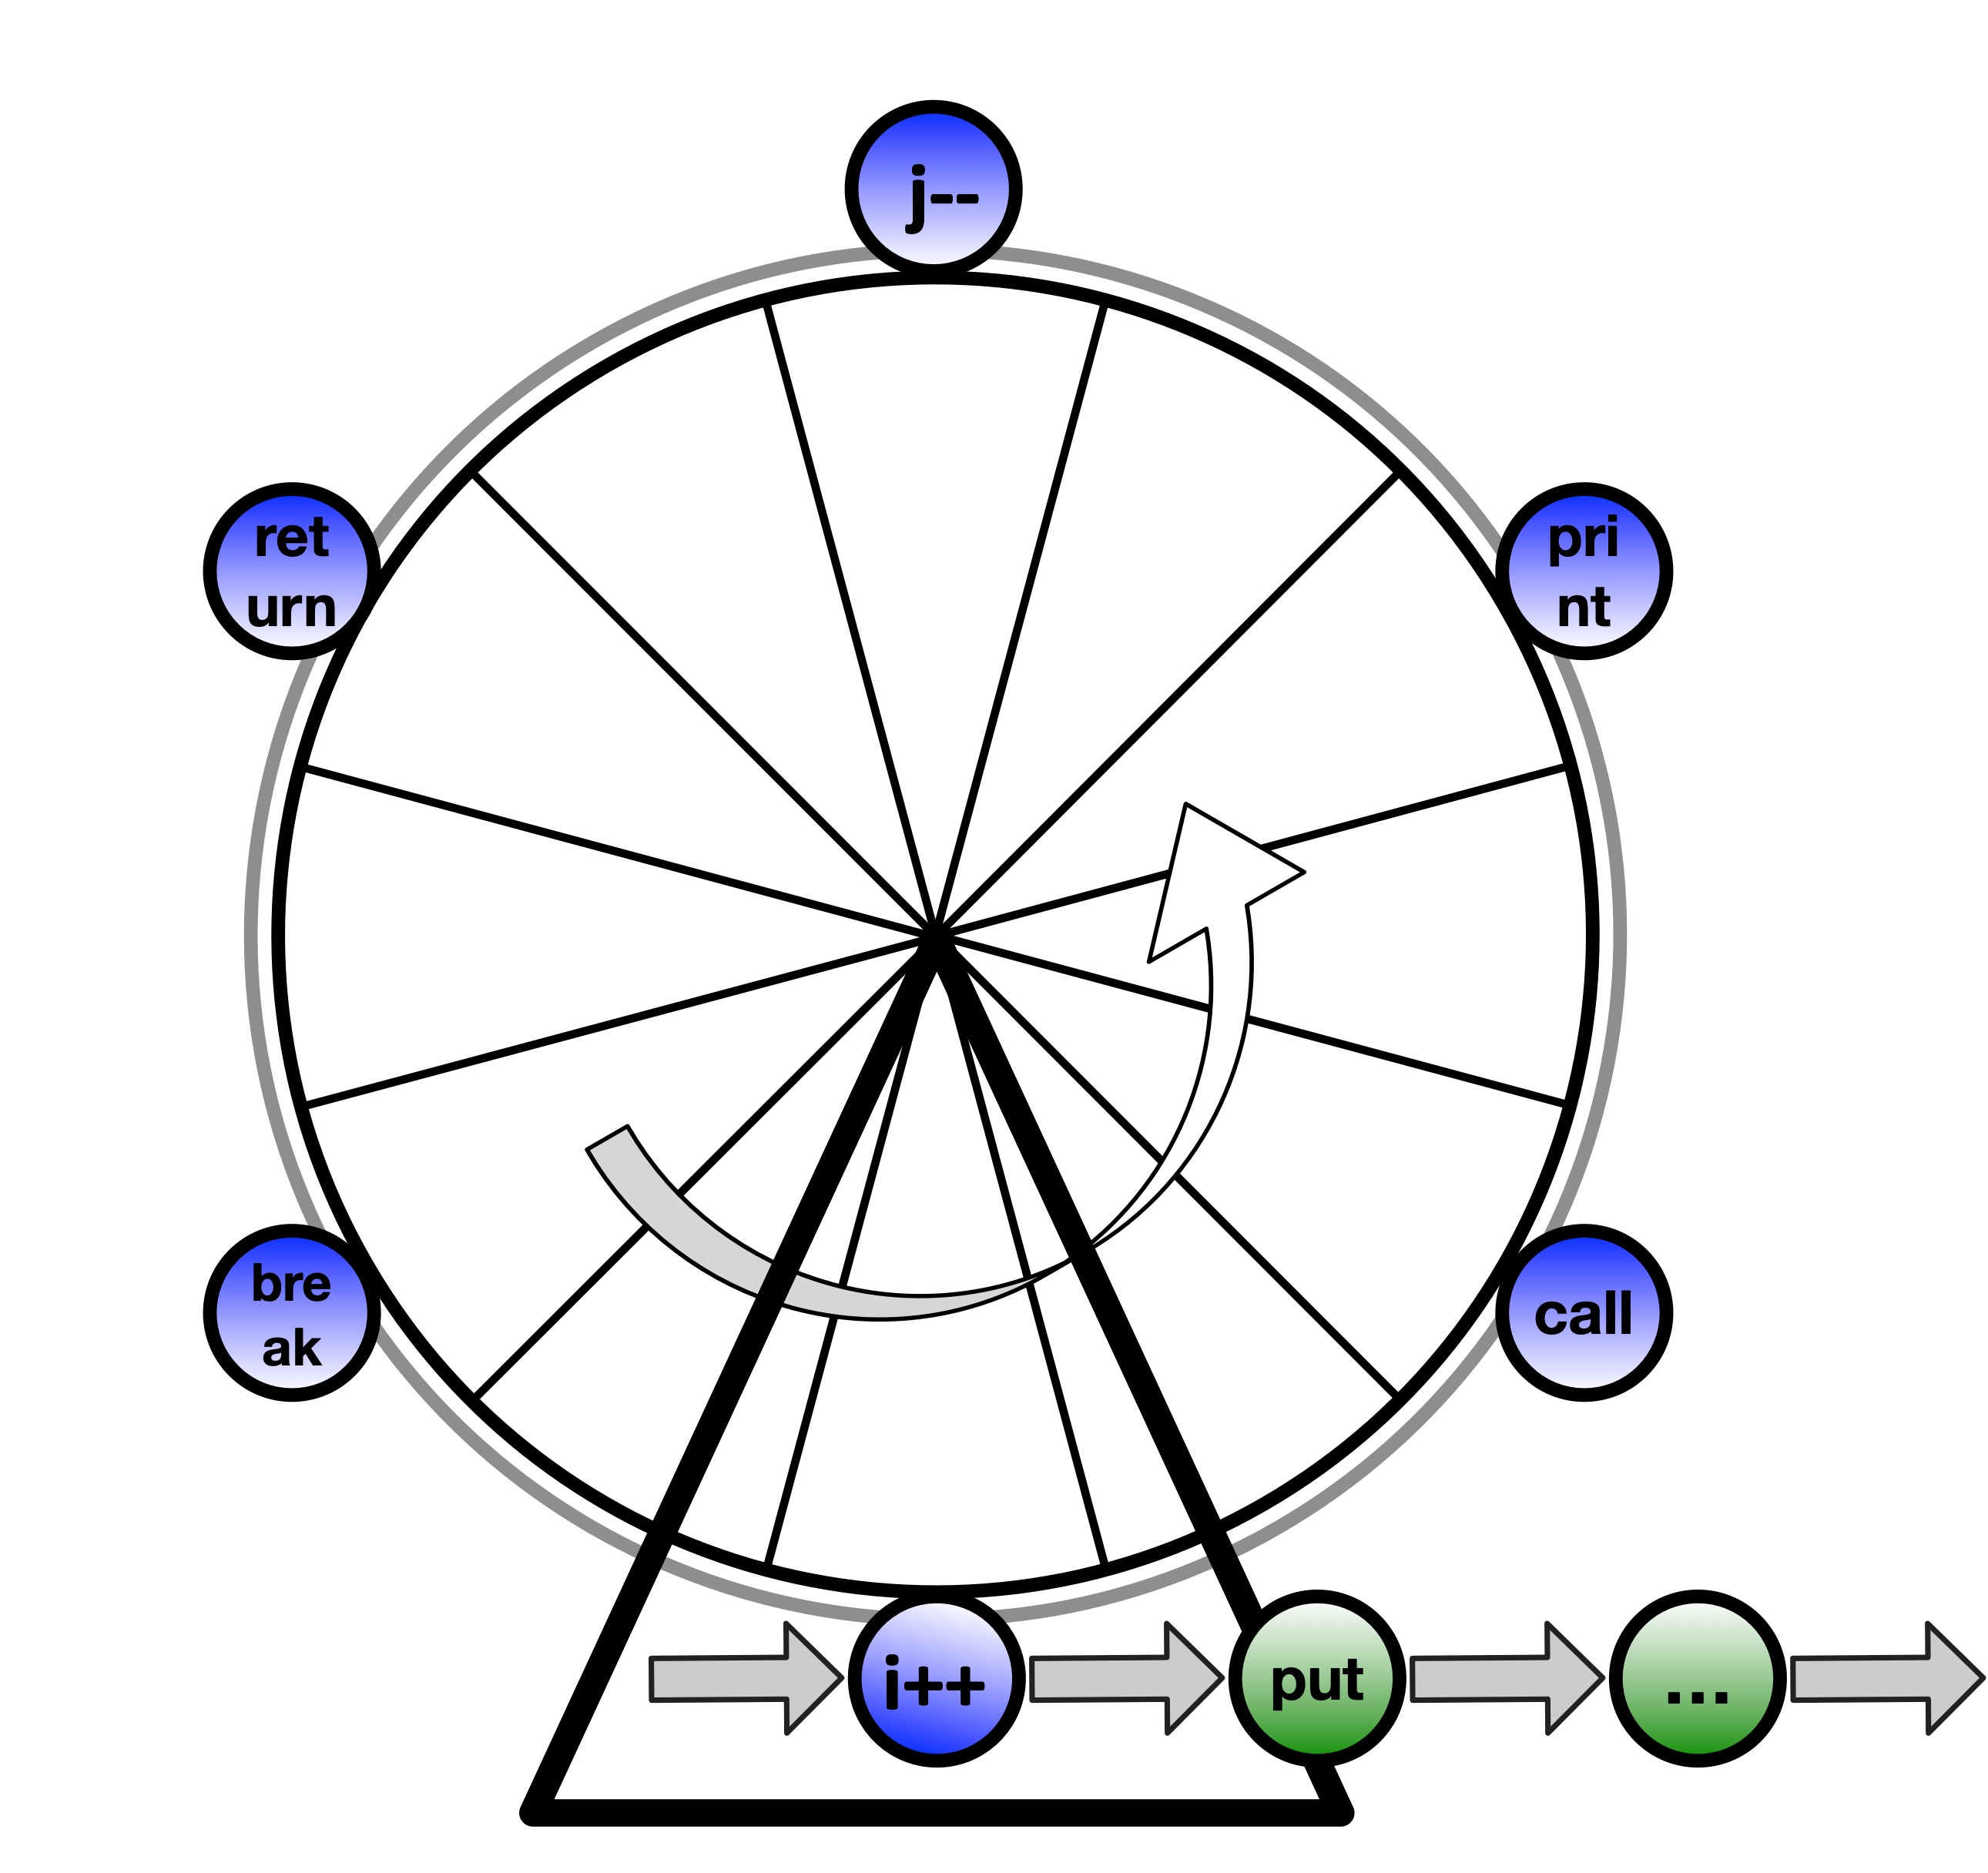
\includegraphics[width=\textwidth]{ferris-wheel-rotated.jpg}
        \caption{\label{fig:ferris-wheel-rotated}}
    \end{subfigure}
    \caption{\label{fig:loop-rotation} Loop as a circular sequence.
    Legend: statements are represented by circular nodes;
    blue ones are loop statements, green ones are non-loop statements.
    The statements ``\code{i++}'' and ``\code{call}'' are duplicated statements between pre-loop
    and loop.
    They can be coalesced into the loop by a loop rotation.
    \protect\subref{fig:ferris-wheel-dup-node}: Original code contains duplicate code;
    \protect\subref{fig:ferris-wheel-rotated}: After rotation, duplicate code is crushed.}
\end{figure}


For example, if the code in the loop and in the vicinity of the loop are duplicate, one may
`rotate' the loop to match up and coalesce the duplicate code.
On the contrary, if one wants to move a portion of the code from the very beginning to the very end
of the loop, one may `reversely rotate' the loop loose.
Doing so will result in duplicate code.
But this may enable a subsequent refactor whose positive effect will eventually pay off this
adverse effect.
In combination, we refer to both operations as `loop rotation'.
In practice, one may start with the more malleable ``\code{while (true)}'' or
``\code{for (; ;)}'' loops.
This will help one focus on coming up with \emph{a} working and flexible code first.
Then one can use the `loop rotation' technique to fine-tune the program.
